\section*{Variational Autoencoders}

\begin{frame}{Introduction to VAE}
    Variational Autoencoders (VAE) have same structure as autoencoders, but here we learn the distribution of the hidden representation, rather than learning the fixed hidden representation.

    \pause 
    \begin{block}{2 things to care about}
        1. We are interested in learning the distribution $P(z^{(i)}|x^{(i)})$ so that we can sample highly likely $z^{(i)}$ for a given $x^{(i)}$.\\
        2. We are also interested in learning the distribution $P(x^{(i)}|z^{(i)})$ so that we can generate new data by sampling $z^{(i)}$ from $P(z^{(i)}|x^{(i)})$.
    \end{block}

    \textcolor{blue}{With above choice, neither encoder nor decoder is deterministic.}
\end{frame}

\begin{frame}{Modelling Assumptions}
    \begin{block}{Assumption 1}
        $z^{(i)} \sim N(0, I_{k \times k})$ \\
    \end{block}

    \begin{block}{Assumption 2}
        Posterior distribution $P(z^{(i)}|x^{(i)}) \sim N(\mu(x^{(i)}), \Sigma(x^{(i)}))$ , where $\mu(x^{(i)})$ and $\Sigma(x^{(i)})$ are the functions of $x^{(i)}$.
    \end{block}

    \begin{block}{Assumption 3}
        $P(x^{(i)}|z^{(i)}) \sim N(\mu(z^{(i)}), \Sigma(z^{(i)}))$ , where $\mu(z^{(i)})$ and $\Sigma(z^{(i)})$ are the functions of $z^{(i)}$.
    \end{block}
\end{frame}

\begin{frame}{Achieving the goals}
    1. Since we assumed that $P(z^{(i)}|x^{(i)}) \sim N(\mu(x^{(i)}), \Sigma(x^{(i)})$, the goal of encoder network is to learn mean and variance of the distribution.\\ 
    \bigskip
    2. We also assumed that $P(x^{(i)}|z^{(i)}) \sim N(\mu(z^{(i)}), \Sigma(z^{(i)})$, the goal of decoder network is to learn mean and variance of the distribution.\\
\end{frame}

\begin{frame}{Visualizing the VAE}
    \begin{figure}
        \centering
        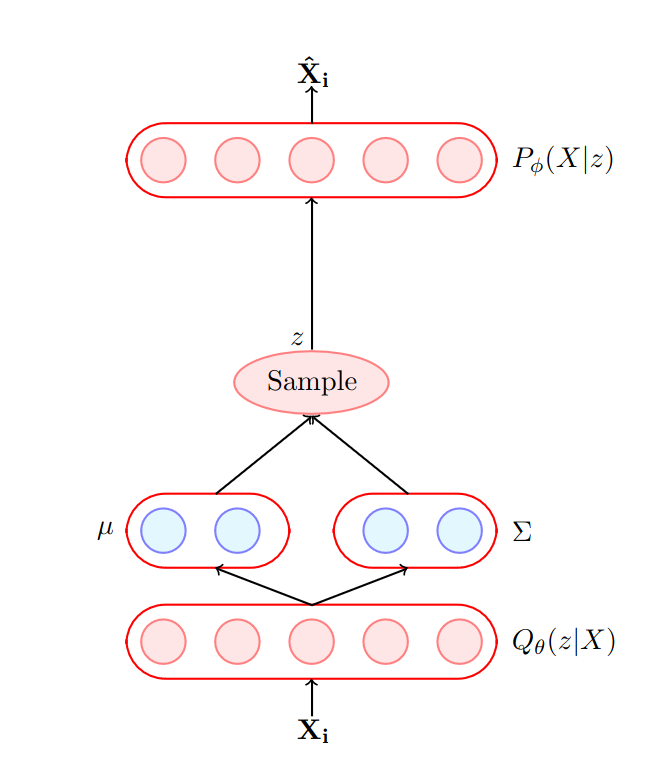
\includegraphics[width=0.4\textwidth]{vae.png}
        \caption{Variational Autoencoder}
    \end{figure}
\end{frame}

\begin{frame}{Loss Function in VAE}
    We optimize the following MSE Loss + KL Divergence Loss where KL Divergence Loss is given by:
    \begin{equation}
        \boxed{KL(P(z^{(i)}|x^{(i)}) || P(z^{(i)})) = \frac{1}{2} \sum_{j=1}^{k} (\mu_j^2 + \sigma_j^2 - \log(\sigma_j) - 1)}
    \end{equation}
    where $\mu_j$ and $\sigma_j$ are the mean and variance of the latent space distribution $P(z^{(i)}|x^{(i)})$.In practice we assume that covariance matrix is diagonal.
    \pause 
    This can be derived from the expression of KL Divergence between two Gaussian distributions.
\end{frame}

\begin{frame}{VAE's on MNIST dataset}
    \begin{figure}
        \centering
        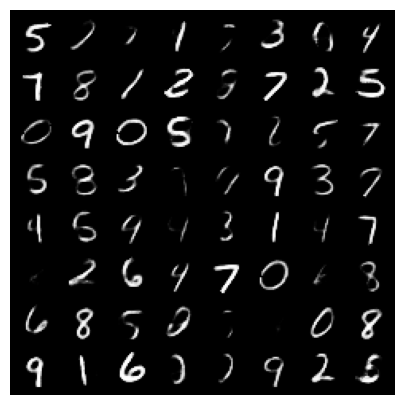
\includegraphics[width=0.4\textwidth]{../ReportNeurips/mnistGenerated1.png}
        \caption{Generation of new handwritten digits using VAE}
    \end{figure}
    We can clearly see that VAE has generated better handwritten digits than autoencoders.
\end{frame}


\begin{frame}{VAE's on MNIST dataset}
    \begin{figure}
        \centering
        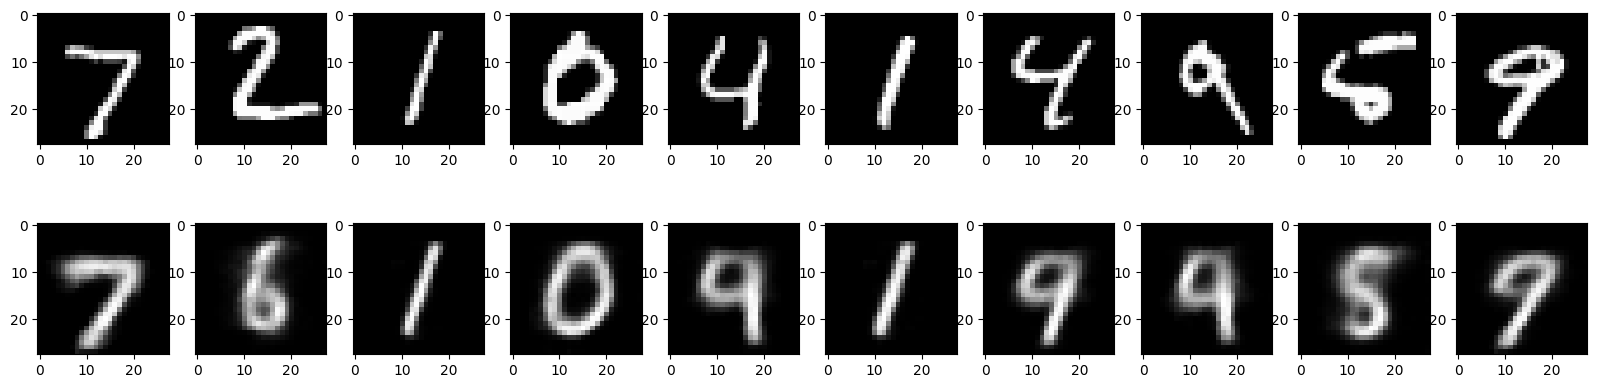
\includegraphics[width=0.8\textwidth]{../ReportNeurips/mnistReconsrtructvae.png}
        \caption{Reconstructions of VAE on MNIST dataset}
    \end{figure}
    Reconstructions are also similar to the original data.
\end{frame}

\begin{frame}{Key observations}
    1. Autoencoders are deterministic, while VAE's are probabilistic.\\
    2. VAE's are better in generating new data than autoencoders.\\
    3. Autoencoders are better in reconstruction than VAE's.\\
\end{frame}

